\documentclass[11pt]{article}
\usepackage{amsmath}
\usepackage{amssymb}
\usepackage{graphicx}
\usepackage{algorithm}
\usepackage{algorithmicx}
\usepackage{algpseudocode}
\usepackage{booktabs}
\usepackage{tabularx}
\usepackage[margin = 1.0in]{geometry}

\begin{document}


\title{An Investigation of Genetics-Based Machine Learning as Applied to Global Crop Yields}
\author{Will Gantt}
\maketitle
\clearpage

\section{Introduction}

% What is the problem that your project is trying to address?
As Earth's population continues to grow and as the effects of climate change intensify, it is critical that we better understand the environmental and economic factors that most significantly affect agricultural output around the world. While rising temperatures may benefit certain crops in the short term, extreme weather and higher levels of atmospheric $\text{CO}_2$ will, if left unchecked, have disastrous consequences for water supply, soil fertility, and, consequently, for crop yields. \cite{us_epa_climate_2017}. Moreover, the United Nations Department of Economic and Social Affairs predicts that the world population will reach 9.7 billion by 2050 and 11.2 billion by the end of the century \cite{noauthor_world_2015}.

% How do you plan to address it?
These forecasts demand prudent planning, which in turn requires that we be able to discern trends in agricultural data. To that end, I have designed and written a learning classifier system (LCS)---a powerful and versatile tool  for data mining---and have applied it to data collected by Erik Nelson in order to probe the relationships between various agricultural inputs and changes in crop yields.
This paper presents the preliminary results of my investigations.

% Outline of rest of paper
The following section gives a brief overview of genetics-based machine learning (GBML) and LCSs, and of the research done by Nelson and Congdon that gave rise to this project \cite{nelson_measuring_2016}. Section 3 provides a thorough description of the system design of my own LCS. Section 4 details the experiments conducted and the results. Finally, section 5 offers some concluding remarks and suggests directions for future work, and section 6 contains experimental data.

\section{Background}

In this section, I provide some context for my project. First, I introduce the GBML paradigm and consider the place of LCSs within it. Next, I give a general overview of LCSs and their basic structure. I then discuss a few important developments in the history of LCSs for supervised learning, and conclude by talking specifically about the earlier work of Nelson and Congdon \cite{nelson_measuring_2016}.

\subsection{Genetics-Based Machine Learning}

GBML is a machine learning approach based on the use of evolutionary computation. Briefly, evolutionary computation comprises a set of optimization algorithms that evolve populations of candidate solutions to a particular problem through a process inspired by biological evolution. Many of the most interesting and important problems in machine learning have large and noisy search spaces, and it is in such contexts that techniques from evolutionary computation have proved particularly effective.

The precise relationships between various GBML-related terms and concepts have changed over the years, and usage in the community is often loose. GBML, once taken to refer exclusively to LCSs, is now considered a broader term that encompasses a number of other algorithms, including genetic programming, evolutionary ensembles, evolutionary neural networks, and genetic fuzzy systems \cite{kovacs_genetics-based_2012}. For the purposes of this paper, it is important only to recognize that LCSs exist within a larger machine learning problem-solving framework.

\subsection{What is a Learning Classifier System?}

\subsubsection{Structure}

Introduced by John Holland in 1975, LCSs are GBML algorithms that evolve a population of rules\footnote{Rules are also frequently referred to as ``classifiers.'' To maintain a clear distinction between individual \emph{classifiers} and the \emph{classifier systems} that comprise them, I use the term ``rule'' exclusively throughout to denote the former, and ``LCS'' to denote the latter.} \cite{holland_adaptation_1975}. Each rule consists of a condition that indicates when the rule applies, as well as an action to take if the condition's criteria are met. As LCSs have applications to a variety of learning problems, the function of the rules depends largely on the task. With supervised learning problems, rules attempt to categorize a set of training examples by mapping the features of those examples to particular classes. In these cases, a rule's condition describes the features of the examples to which it applies, and the action specifies the class to be assigned to examples matching the condition. Problems in reinforcement learning, by contrast, often involve determining the best action for an agent to take in response to certain inputs or stimuli from the environment. Here, a rule's condition describes a set of inputs and its action determines how the agent should react given those inputs.

Regardless of the types of problems to which they are applied, all LCSs share certain basic structures and mechanisms. Holmes et al. have identified four such components  \cite{holmes_learning_2002}, but their model is more characteristic of LCSs used in reinforcement learning than those used in supervised learning. I suggest a slight modification of that model that covers both:
\begin{enumerate}
\item \emph{Population.} All LCSs have a population of rules. Although some systems allow for the growth or reduction of the population, there is typically a limit on the maximum number of rules it may contain.
\item \emph{Learning.} An LCS must have a means of coercing its population toward rules that generate good actions or accurate classifications. Numerous methods have been used for this purpose and they tend to vary based on the kind of learning. Many early LCSs designed for reinforcement learning used the bucket brigade algorithm \cite{holland_properties_1985}, while more contemporary systems often rely on Q-learning \cite{c._j._c._h._learning_1989, orriols-puig_fuzzy-ucs:_2009} or Q-learning-inspired algorithms. For supervised learning tasks, other systems have used genetic algorithms exclusively \cite{llora_towards_2007}. Still others have used different approaches, including ensemble learning \cite{gao_learning_2005} and bayesian methods \cite{hai_h._dam_bcs:_2006}.
\item \emph{Discovery.} An LCS must also have mechanisms for generating new rules. For that purpose, a vast majority of systems employ genetic algorithms (GAs), which provide two useful operations: crossover and mutation. Crossover produces two ``offspring'' rules from two existing ``parent'' rules, and mutation alters some of the attribute values of the offspring. But many LCSs employ additional operators. The \emph{covering} operator, for example, which creates a new rule when there are none that match the current input, has been widely used \cite{orriols-puig_fuzzy-ucs:_2009, wilson_classifier_1995, bernado-mansilla_accuracy-based_2003}. \emph{Specify}, a second popular operator, proposed by Pier Lanzi,  attempts to counteract the over-generalization of rules by specifying the attribute values of a rule according to a particular input \cite{lanzi_study_1997}. 
\item \emph{Classification or Action Selection.} Finally, an LCS must have some procedure for deciding what action to take or how to classify a particular example. In the typical case, the action or classification is selected based on the actions recommended by the rules in the \emph{match set}---the set of rules matching a particular input. One possibility is simply to choose the action of the fittest rule in the match set. Another is to conduct a weighted vote of all the rules in the set, where each rule casts a ``vote'' for its action, weighted by its fitness. The selected action, then, is the one receiving the greatest number of points. Some systems have also incorporated random action selection alongside one of the first two methods \cite{wilson_classifier_1995}.
\end{enumerate}

These are, at the broadest level, the modules that feature in all LCSs. There is, of course, substantial variation between implementations, which is to be expected of a paradigm with applications as diverse as those of the LCS algorithm.

\subsubsection{Genetic Algorithms}

As GAs constitute such a critical component of LCSs, they merit at least a short and very general overview. GAs evolve populations of candidate solutions to a particular problem by a process inspired by biological evolution. In a traditional implementation, individuals are represented as bit strings, where each index in the strings corresponds to a particular property of the solution and a 1 or 0 at that index indicates the presence or absence of the property, respectively. In LCSs, a third character (a ``don't care'' value, often denoted by ``\#'') is often used to indicate that the property is not relevant for a given rule. In principle, solutions may take any form, and GA variants have been developed to accommodate structures of different kinds, including objects \cite{keijzer_evolving_2001}. The canonical GA works as follows\footnote{For ease of illustration, I have used bit strings as the solution type in this example.}:
\begin{enumerate}
\item \emph{Initialization.} Generate a random population of candidate solutions.
\item \emph{Evaluation.} Evaluate the fitness of each individual according to some fitness function.
\item \emph{Selection.} Select $n$ individuals from the population to reproduce. The probability that a given individual will be selected is usually proportional to its fitness.
\item \emph{Crossover.} Randomly pair the $n$ selected individuals. For each pair, combine the bits of one member of the pair with those of the other (e.g. via one-point crossover) to produce two new solutions (``offspring'').
\item \emph{Mutation.} Flip some number of the bits of each of the offspring with probability $p$.
\item \emph{Replacement.} Replace the $n$ least-fit members of the original population with the offspring created in (5).
\item Repeat (2)-(6) until the stopping condition (e.g. a target average fitness, a specific number of generations, or a runtime limit) is met.
\end{enumerate}
The structure of the GA is just one respect in which different implementations of LCSs can differ. The next section outlines a second.

\subsubsection{Pittsburgh and Michigan Styles}

One of the most common and useful categorizations of LCSs distinguishes between \emph{Michigan-} and \emph{Pittsburgh-} or \emph{Pitt-style} systems. The difference pertains to what counts as an ``individual'' in the population. In Michigan systems, an individual is a single rule. In Pitt systems, however, an individual is an entire rule \emph{set}. Correspondingly, a solution in a Michigan system often comprises the entire population, while a solution in a Pitt system consists of a single individual (a rule set). This difference has important implications for many aspects of LCS design, including the learning algorithm, credit assignment, rule syntax, and genetic operators. Perhaps unsurprisingly, each style has notable advantages and disadvantages with respect to the other. Michigan systems, for example, typically require less memory and are less computationally intensive, while Pitt systems avoid the difficulties involved in distributing credit across individual rules. Neither type has emerged as obviously superior to the other, but Michigan systems do appear to predominate in the literature \cite{urbanowicz_learning_2009}.

\subsection{Developments in LCS Research}

Numerous thorough histories and comparisons of LCS research have been written over the years \cite{urbanowicz_learning_2009, lanzi_roadmap_2000, wilson_critical_1989, wilson_state_2000}, and it is beyond the scope of this paper to undertake another one. Instead, I wish to highlight just a few key milestones in the particular domain of LCS research with which my project is concerned---namely, supervised learning and data mining. Each of the systems listed introduced at least one important concept to that domain.

\subsubsection{LS-2}

Schaffer and Grefenstette's LS-2 \cite{schaffer_multi-objective_1985} was the first attempt to use an LCS for a genuine supervised learning classification task. Specifically, they applied their system to the multi-class problem of classifying five human gait types based on EMG signals from the leg muscles. A total of 11 training examples were used, and rules were represented as 12-bit strings from the ternary alphabet $\{0,1,\#\}$, with each index representing a particular signal.

LS-2 evolved a population of rule \emph{sets} and may thus anachronistically be categorized as a Pitt-style LCS, though the distinction had yet to be formulated when the article was published. Of particular note in this system is the fitness scheme. LS-2 represented fitnesses, not as scalar quantities, but as vectors whose elements corresponded to the different possible classes (gait types). For each rule set, a fitness vector was computed as a function of the number of correctly and incorrectly classified examples in each class. When constructing the population for the next generation, a portion of the rules were selected on the basis of each element in the fitness vector. In allowing fitness to be relativized to individual classes, Schaffer and Grefenstette introduced the notion of \emph{niching}---the specialization of rules to particular regions of the solution space---which  featured heavily in later systems, and which remains a critical topic in contemporary research.

\subsubsection{FCS}

Many kinds of data in the real world have continuous-valued attributes. Given the traditional bit string rule representation of an LCS, determining the best way to handle data of this sort is a challenge. In 1991, Manuel Valenzuela-Rend\'on proposed a solution to this problem using fuzzy sets \cite{manuel_valenzuela-rendon_fuzzy_1991}. In fuzzy set theory, the membership of an element in a set is determined by a membership function. Defining membership in this way allows for elements to be \emph{partial} members of sets.

Valenzuela-Rend\'on's ``fuzzy classifier system'' (FCS) applied this logic to rule representation. Suppose the condition of a rule $R$ contains a ``temperature'' attribute, whose possible values are ``cold,'' ``mild,'' and ``hot.'' Instead of assigning $R$ one of those values, FCS would define a membership function for each value, and $R$ would be assigned some combination of those functions. If, for example, $R$ was assigned the functions for ``cold'' and ``mild,'' the result would be a curve for the temperature attribute that, given a real-valued temperature, indicated the \emph{degree} to which that temperature should be considered ``cold'' or ``mild.''

In short, structuring rules in this way introduced two valuable concepts to the LCS community: (1) the ability of LCSs to handle real-valued inputs, and (2) the possibility of eliminating hard boundaries between classes.

\subsubsection{XCS}

Although designed explicitly for reinforcement learning, the ``eXtended Classifier System'' (XCS), proposed by Wilson in 1995, exerted such a profound influence on LCS research of all kinds that it deserves mention here \cite{wilson_classifier_1995}. Nearly all of the key features of XCS had been implemented in earlier systems, but its impressive accuracy and generalization capabilities made clear for the first time the potential effectiveness of those features.

XCS pioneered a slew of techniques that have since become staples of LCS design, particularly in reinforcement learning, including the use of Watkins's Q-learning algorithm for credit assignment and the use of a niche GA \cite{urbanowicz_learning_2009}. However the technique of greatest relevance to supervised learning was the use of accuracy-based fitness. Wilson was not the first to use accuracy-based fitness (the credit goes to Holland and his first LCS, CS-1 \cite{holland_cognitive_1977}), but a substantial majority of previous systems used a different parameter known as \emph{strength}. Strength was decidedly a reinforcement learning mechanism, and measured the expected reward (or ``reward prediction'') from the environment if the action of a particular rule was taken. The problem with strength-based fitness was that it tended to eliminate rules that predicted lesser rewards, but that nonetheless reliably led to the best action in specific circumstances. Even though accuracy had been used before, XCS radically increased its popularity and is now considered the primogenitor of all contemporary accuracy-based systems \cite{urbanowicz_learning_2009}.

\subsubsection{UCS}

In 2003, Bernad\'o-Mansilla and Garrell-Guiu presented a supervised learning variation on XCS \cite{bernado-mansilla_accuracy-based_2003}. Dubbed ``UCS,'' their system adapted the reinforcement learning model of XCS to better suit multi-objective classification tasks. UCS retained all of the main features of XCS, including its accuracy-based fitness scheme, a GA that encouraged niching, and an online learning style, but it changed the manner in which accuracy was computed. The details of the differences are not salient; rather, the significance of UCS consists in its demonstration that ideas from reinforcement learning within LCS research could, with some effort, be refashioned to yield good solutions to problems in supervised learning.

\subsection{Global Crop Yields}

The remainder of this section summarizes the research conducted by Erik Nelson and Clare Bates Congdon in \cite{nelson_measuring_2016}. Their work --- and mine --- examines data on crop yields collected by Nelson and his students in the economics department. The data relate various environmental and economic variables to the agricultural output of countries, both in units of mass (Mg/ha) and in units of energy (Mkcal/ha), from 1975 to 2007. The variables considered cover such categories as growing season weather; crop choice; investment in irrigation capability, land, and machinery; agricultural technology; fertilizer use; and cropped footprint. 

Using these data, Nelson and Congdon evaluated the relative impact of the year-to-year changes in the different variables on the change in global and regional crop yields \cite{nelson_measuring_2016}. The authors applied two analytical methods: fixed-effects econometric modeling and decision trees, each of which is explained in greater depth below. For both, annual changes in yield were discretized to the categories ``high'' (H), ``medium'' (M), and ``low'' (L). 


% Fixed-Effects Modeling
\subsubsection{Fixed Effects Modeling}

Fixed-effects models offer a means of accounting for any unobserved, time-independent factors that affect a dependent variable in the analysis of panel data---that is, multi-dimensional data containing measurements across time. In Nelson and Congdon's work, the dependent variables considered were the per-hectare crop yield in metric tons (Mg) and in millions of kilocalories (Mkcal). Let $y_{ct}$ be the per-hectare crop yield (in whichever units) for a country $c$ in a year $t$. The fixed effects model, then, has the form
$$y_{ct} = \beta_1x_{ct1} + \beta_2x_{ct2} + \ldots + \beta_Nx_{ctN} + \mu_{ct} + a_c$$
Where $x_{cti}$ is the value of the independent variable $x_i$ for country $c$ in year $t$; $\beta_i$ is the coefficient for the independent variable $x_i$; $\mu_{ct}$ (the ``idiosyncratic error'') covers all unobserved, time-\emph{variant} effects  on $y_{ct}$; and $a_c$ (the ``fixed effect'') captures all unobserved and time-\emph{invariant} effects.
The specific variables used are shown in table \ref{vars} (as above, the subscript ``$_{ct}$'' indicates that the variable is for a country $c$ in a year $t$).

\begin{table}
\begin{tabularx}{\textwidth}{cl}
\toprule
Variable & Description \\
\midrule
$\pmb{X_{ct}}$ & a vector of harvested hectare percentages across different crops. \\
$\pmb{K_{ct}}$ & a vector of variables measuring investment in agricultural \\
& machinery and equipment per harvested hectare. \\
$A_{ct}$ & the total harvested hectarage. \\
$S_{ct}$ & the soil quality. \\
$I_{ct}$ & the percentage of harvested land equipped for irrigation. \\
$\pmb{Z_{ct}}$ & a vector of various annual weather statistics. \\
$F_{ct}$ & the total amount of fertilizer used. \\
\bottomrule
\end{tabularx}
\caption{Variables used in Nelson and Congdon's analysis of crop yield data \cite{nelson_measuring_2016}}
\label{vars}
\end{table}

Thus, their fixed effects model, computed using the method of least squares, has the form
$$Y_{ct} = \beta_0 + \pmb{\beta_1}\pmb{X_{ct}} + \pmb{\beta_2}\pmb{K_{ct}} + \beta_3A_{ct} + \beta_4S_{ct} + \beta_5I{ct} + \beta_6\pmb{Z_{ct}} + \beta_7t + \beta_8F_{ct}$$

Using this model, the authors constructed expected yield curves for each country between 1975 and 2007 (in both Mg/ha and Mkcal/ha), as well as for the temperate and tropical regions, and for the world. They also constructed counterfactual yield curves for each country and for each variable, by holding that variable constant at 1975 levels. By comparing the integral of an expected yield curve with the integral of a corresponding counterfactual curve for a variable $v$, one can evaluate the impact of $v$ on yield relative to other variables.

% Decision Trees
\subsubsection{Decision Trees}

Decision trees are machine learning tools for classification that, much like LCSs, attempt to group the outcomes of a process based on the inputs to that process. In this case, the outcomes are simply the changes in country-level crop yields and the inputs are the year-to-year changes in the values of the variables listed above. Each node in the tree corresponds to an attribute of the input (e.g. change in soil quality) and specifies a value of that attribute according to which the training examples may be partitioned into two groups: examples whose value for that attribute falls above the specified value and those whose value is less than or equal to the specified value. Beginning at the root node and partitioning in this way generates some number of leaves, each containing a subset of the examples. The objective is to construct a tree such that the examples in each leaf are as homogeneous as possible with respect to their outcomes. A path from the root node to one of the leaves thus characterizes the attribute values of the examples in that leaf. The closer to the root an attribute node is, the more it may be said to ``explain'' the differences in outcomes among the examples.

% Results
\subsubsection{Results}
Both methods found that changes in crop mix accounted for more of the growth in yield between 1975 and 2007 than any other single variable. In the tropics, an increase in the average daytime growing season temperature correlated with a noticeable decrease in yields. Perhaps surprisingly, investment in irrigation, land, and machinery and equipment, as well as the quality of the cropped soil, had a negligible impact. The methods disagreed, however, on the importance of fertilizer use: Where the econometric model showed it to have a significant positive influence on yields, the decision trees revealed no such relationship.

% Why use LCSs?
With all of this analysis already done, one may reasonably question the utility of re-evaluating the same data with an LCS. There are at least two advantages:

\begin{enumerate}
\item LCSs have proved themselves effective in supervised learning tasks of precisely this sort and have the potential to reveal important patterns in the data not made evident by either decision tree or regression analysis.
\item An LCS may offer further support for the findings obtained through these first two methods.
\end{enumerate}

\section{System Design}

In this section, I present my design for a Michigan-style LCS for the classification of examples with real-valued attribute vectors. The explanation consists of four parts: The first part explains the representation of rules, including a short description of their attributes, and a longer discussion about the choice of representation of the condition in particular. The second part describes the learning component and offers a general overview of the GA, as well as more detailed analysis of its constituent modules. The third part covers the testing component---the algorithm for the classification of new examples once a rule set has been created. Finally, the fourth part enumerates the parameters of the LCS.

\subsection{Rule Representation}

Rules are represented as objects with the following member variables:

\begin{description}
\item \textit{id}: A unique identifier for the rule in the population.
\item \textit{classification}: The class, given by an integer value, that an example matching the rule will be assigned.
\item \textit{true\_positives}: The number of examples that the rule both matches and correctly classifies.
\item \textit{true\_negatives}: The number of examples that are neither matched by the rule nor of the same class.
\item \textit{false\_positives}: The number of examples that the rule matches, but incorrectly classifies.
\item \textit{false\_negatives}: The number of examples that have the same class as the rule but that the rule does not match.
\item \textit{num\_dont\_care}: The number of Attribute objects in the rule's condition (represented as a vector of Attribute objects) whose \textit{dont\_care} variable is currently set to true.
\item \textit{fitness\_1}: An initial fitness value used to determine a preliminary ranking of the rules.
\item \textit{fitness\_2}: A fitness value that is based on Fitness 1, but that takes into account redundancy (the covering of examples already covered by other, fitter rules).
\item \textit{condition}: A vector of Attribute objects that describes the attribute values an example must have to be matched by the rule.
\end{description}

As mentioned in section 2.2.2, much of LCS research has concerned itself with the classification of examples with binary-valued attributes that simply indicate the presence or absence of some feature in the example. The conditions of rules used in LCSs of this sort may therefore be represented as strings of characters from the ternary alphabet $\{0,1,\#\}$. But when dealing with real values, determining how best to represent the condition is more difficult. With real values, not only does the search space expand to a theoretically infinite size, but the genetic operators (crossover and mutation) have to be adapted as well. Thus, the condition must be constructed in a manner that (a) reduces the search space to a reasonable size, and (b) does not hinder or over-complicate the functioning of the genetic operators.

The success of fuzzy LCSs like FCS \cite{manuel_valenzuela-rendon_fuzzy_1991} and Fuzzy-UCS \cite{orriols-puig_fuzzy-ucs:_2009} (a fuzzy update of the original UCS) suggests one promising approach. Given the complexity of these sytems, though, and time limitations, I chose the simpler, but nonetheless well-supported method of discretizing all attributes into some number of quantiles. Each attribute in the rule's condition not marked as irrelevant covers a range of values specified by one of the quantiles. Note that a condition constructed in this way meets both of the criteria given in the preceding paragraph: It radically restricts the search space (since each attribute will have a small number of quantiles) and it does not inhibit or fundamentally alter the behavior of the genetic operators (as will be shown in more detail further on in this section). The number of quantiles used is the same across all condition attributes and is specified by the user. The condition is represented as a vector of Attribute objects, each of which has a name, a quantile number, an upper and lower bound describing the range of that quantile, and a boolean ``don't care'' value indicating whether the attribute is relevant for the rule to which it belongs.

\subsection{Rule Discovery and Learning}

\subsubsection{Overview}

As with virtually all other LCSs, this system uses a GA in its discovery component. One complete run of the LCS attempts to characterize a single ``target'' class from the data. The population is initialized with a user-specified number of rules whose class attribute (action) values are set to that of the target class, and whose condition attributes are randomly either marked as irrelevant (i.e. with their \textit{dont\_care} variables set to true) or else assigned a random quantile. For each rule in the population, the system tallies the number of true positives, true negatives, false positives, and false negatives among the examples in the training set. The rule is then assigned a preliminary fitness by computing the natural log of the odds ratio and adding a small boost for each of its attributes that is marked as a ``don't care.'' Once this has been done for the entire population, the rules are ranked by fitness. 

Next, a second fitness is calculated using the same procedure, except that an example may count as a true positive for at most one rule. In computing the original fitness, it frequently happens that a single example will be counted as a true positive for multiple rules. In order to avoid such redundancy and to encourage diversity in the population, the second fitness counts an example as a true positive only for the fittest rule (based on the first fitness) that covers it. 

The $N$ best rules as evaluated by this second fitness are then immediately added to the next generation. To fill the remainder of the new population, $pop\_size - N$ rules are selected for reproduction from the current one using stochastic universal sampling. The selected rules are paired and crossed over to produce two offspring, which are mutated and added to the next generation. The process then repeats for a user-specified number of iterations.

\subsubsection{Fitness Update}

Both the first and second fitnesses are computed using the natural log of the odds ratio, in conjunction with a slight bonus for each of its ``don't care'' attributes. A given example is either a positive instance ($T+$) of the target class or a negative instance ($T-$). Similarly, a given rule will \emph{classify} the example either as a positive instance of the target class ($R+$) or a negative instance ($R-$). The four possible combinations of the example's actual class \mbox{($T+/T-$)} and the class that a given rule selects for that example ($R+/R-$) yield the following matrix:

\begin{figure}[h!]
\centering
\begin{tabular}{c|cc}
& $T+$ & $T-$ \\
\hline
$R+$ & $a$ & $b$ \\
$R-$ & $c$ & $d$ \\
\end{tabular}
\caption{The matrix of true positives, true negatives, false positives, and false negatives. The column indicates whether an example is a positive or negative instance of the target class. The row indicates whether the rule classifies the example as a positive or negative example.}
\label{odds_ratio}
\end{figure}
Clockwise from the top left, the elements of the matrix correspond to true positives, false positives, true negatives, and false negatives (for a given rule and example pair). As its name suggests, the odds ratio is a ratio of two odds:

\begin{enumerate}
\item The odds that a rule classifies an actual positive example of the target class as a true positive ($a/c$).
\item The odds that a rule classifies a negative example of the target class as a true positive ($b/d$).
\end{enumerate}
Dividing (1) by (2) gives:
$$\frac{\Big(\frac{a}{c}\Big)}{\Big(\frac{b}{d}\Big)} = \frac{ad}{bc} = \frac{|TP| \cdot |TN|}{|FP| \cdot |FN|}$$
Note that when either $|FP|$ or $|FN|$ is 0, the odds ratio is undefined. In order to avoid this problem, $|TP|$, $|TN|$, $|FP|$, and $|FN|$ are all initialized to 0.5.

There is no difference in the calculation of the two fitnesses---only in the tallying of true and false positives and negatives. In the first fitness, an example $e$ counts as a true positive for all the rules that match it. In the second fitness, $e$ counts as a true positive only for the \emph{fittest} rule that matches it, as determined by the first fitness. For a rule $R$ that matches $e$, but that is not the fittest that does so, $e$ is simply not included in any of the tallies. Because the second fitness is the one that drives the genetic algorithm, rules that are redundant---that cover examples already covered by fitter rules---will over time be weeded from the population. Observe that this schema also rewards rules that cover just a few examples, so long as those examples are not covered by fitter rules.

Finally, the odds ratio is transformed into log-space to reduce the difference between the fitnesses of the best and worst rules. If the number of true positives and negatives exceeds the number of false positives and negatives by a considerable margin, and if there are many examples in the data set, the odds ratio can become disproportionately large. Taking the log thus preserves diversity in the population by mitigating the dominance of the fittest individuals.

\subsubsection{Selection}

Selection is done based only on the second fitness using stochastic universal sampling (SUS), a superior alternative to traditional roulette wheel selection developed by James Baker \cite{j_reducing_1987}. In roulette wheel (or fitness-proportionate) selection, members of a population are selected randomly, where the probability that a member $k$ is chosen is given by
$$ \frac{\text{Fitness($k$)}}{\sum_{i=1}^N\text{Fitness($i$)}}$$

The basic algorithm is shown on the next page. First, the sum of the fitnesses of all members of the population is computed. Next, a number $r$ in the range $[0, fitness\_sum]$ is determined by randomly selecting a value from the interval $[0,1]$ and multiplying that value by the sum of the fitnesses. The algorithm then iterates over the members of the population. At each iteration, the fitness of the current member is subtracted from $r$. The member whose fitness, when subtracted from $r$, causes $r$ to fall to or below 0 is the one selected. It is clear, therefore, that the larger the fitness of an individual, the more likely it is to be chosen.

\begin{algorithm}
\caption{: Roulette Wheel Selection}
\label{rws}
\begin{algorithmic}
\Function{RWS}{$Pop, N$}
\State $fitness\_sum \gets \text{sumFitnesses}(Pop)$
\State $r \gets$ random($0,fitness\_sum$)
\For{$i \textbf{ in } \{0,\ldots,N-1\}$}
\State $r \gets (r - \text{Fitness($Pop[i]$)})$
\If{$r \leq 0$}
\State \Return{i}
\EndIf
\EndFor
\State \Return{$N-1$}
\EndFunction
\end{algorithmic}
\end{algorithm}

\begin{algorithm}
\caption{: Stochastic Universal Sampling}
\label{sus}
\begin{algorithmic}
\Function{SUS}{$Pop, N$}
\State $fitness\_sum \gets \text{sumFitnesses}(Pop)$
\State $pointer\_dist \gets fitness\_sum/N$
\State $pointer\_start \gets$ random($0,pointer\_dist$)
\State $pointers \gets \text{newArray($N $)}$
\For{$i \textbf{ in } \{0,\ldots,N-1\}$}
\State $pointers[i] \gets pointer\_start + (i \cdot pointer\_dist)$
\EndFor
\State $selected \gets \text{newArray($N$)}$
\For{$p \textbf{ in } pointers$}
\State $j \gets 0$
\While{$\text{sumFitnesses($Pop[0],Pop[j]$)} < p$}
\State $j \gets j + 1$
\EndWhile
\State $selected.\text{Add($Pop[j]$)}$
\EndFor
\EndFunction
\end{algorithmic}
\end{algorithm}

The primary shortcoming of roulette wheel selection is the extent to which it is biased against rules of lesser fitness. Generally speaking, we want the rules selected to be among the fitter ones, but in order to avoid premature convergence, some low-fitness rules must participate regularly in the crossover.

SUS reduces this bias. Instead of generating a new random value for each selection, SUS uses a single random value to make all of its selections. This turns out to be of great utility in increasing the frequency with which low-fitness rules are selected.
Furthermore, it has been shown to have faster average runtime and less variance in the fitnesses of the selected rules than does roulette wheel selection \cite{tobias_blickle_comparison_1995}.

\begin{figure}[h!]
\centering
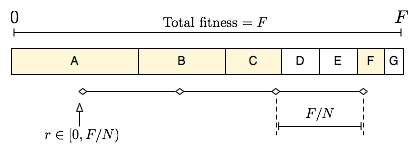
\includegraphics[scale=0.6]{images/sus.png}
\caption{Beginning at a random starting point, stochastic universal sampling (SUS) uses evenly spaced pointers to select rules (Source: \cite{assumed_diagram_2007})}
\label{sus_graphic}
\end{figure}

Algorithm \ref{sus} shows SUS in pseudocode. It will help, in understanding the behavior of SUS, to imagine the interval $[0, fitness\_sum]$ on the real number line. Additionally, imagine that each member of the population is given its own subinterval within the $[0, fitness\_sum]$ that is equivalent in length to its fitness (see figure \ref{sus_graphic}).

To begin, a value known as the ``pointer interval'' is computed by dividing the sum of the fitnesses (\emph{fitness\_sum}) by the number of rules to be selected ($N$). Then, a random number $r$ is chosen from the range $[0, pointer\_interval]$. Beginning at $r$, the algorithm selects $N$ positions along $[0, fitness\_sum]$ by counting out intervals of length $pointer\_interval$. The rules corresponding to the subintervals in which the positions fall are the ones selected.

\subsubsection{Genetic Operators and Replacement}

At each iteration, a fixed number of the fittest rules from the previous generation are added to the next generation. This number is expressed as a fraction of the population size in the \emph{elitism\_rate} parameter, and the rules thus selected are said to be ``elite.'' The rest of the population for the next generation is filled via crossover and mutation of the rules chosen to reproduce during the selection phase.

\emph{Crossover}. The GA uses single-point crossover. For every set of parents, a random integer in the range $[1, num\_attributes - 1]$ is selected as the crossover point. The condition of each of the offspring rules is created by swapping the attribute values to the right of the crossover point in each of the parents. The values of the attributes' \emph{dont\_care} variables are also preserved.

\emph{Mutation}. After crossover, the mutation operator iterates over the condition attributes of each offspring. Each attribute has the same probability of being modified (\emph{p\_mutate}). If it has been determined that an attribute is to be mutated, a second random number in the interval $[0,1]$ is generated. If that number is less than or equal to a probability \emph{p\_dont\_care}, the attribute's \emph{dont\_care} variable is set to true. If the number is greater than \emph{p\_dont\_care}, the attribute is randomly assigned a new quantile.

After both operators have been applied, all of the offspring replace all of the non-elite ($pop\_size - N$) members of the current generation. The resulting population will be the one used in the next generation.

\subsection{Classification of Examples}

The classification of examples in the test set is very straightforward. At the end of \textit{num\_iters} generations, the genetic algorithm terminates. Only the rules in the final population that (a) are elite and that (b) have more true positives than false positives are used for the classification task. There are several reasons for these criteria:
\begin{enumerate}
\item The elite rules in the final population are (mostly) those that have weathered repeated applications of the selection procedure and have proved themselves effective. Among the non-elites, which will have just been generated through crossover and mutation on the final iteration, there are likely to be many bad rules.
\item We are interested in minimizing the number of rules needed to accurately characterize the target class.
\item Rules that incorrectly identify negative instances more frequently than they correctly identify positive ones contribute would only diminish the accuracy of the system.
\end{enumerate}

The number of rules used for the classification may therefore never exceed $pop\_size * elitism\_rate$. Once these rules have been identified, the LCS iterates over the examples in the test set. If a rule that covers the current example is found among the set selected, the example is classified as a member of the target class. If no matching rule is found, the example is classified as a member of the default class.\footnote{Since the system attempts to characterize just one class per run (the target class), it does not matter what is chosen for the default class, so long as it is different from the target class.} After a class has been selected for the example, the system compares the selected class with the actual class of the example and categorizes it accordingly as a true positive, true negative, false positive, or false negative. The tallies of all four categories are outputted once all examples have been classified.

\subsection{Parameters}

The system takes the following arguments:

\begin{description}
\item \textit{pop\_size:} the number of rules in the population.
\item \textit{num\_iters:} the number of iterations the LCS will run before terminating.
\item \textit{target\_class:} the class in the training data that the LCS will attempt to characterize.
\item \textit{elitism\_rate:} the approximate fraction of the population that is to be retained from one generation to the next.
\item \textit{p\_mutate:} the probability that a condition attribute will be mutated when the mutation operator is invoked.
\item \textit{p\_dont\_care:} if it has been determined that an attribute is to be mutated, the probability that its \textit{dont\_care} variable will be set to true (instead of assigning it a new quantile).
\item \textit{training\_set:} a Dataset object containing all of the examples in the training set and other relevant information.
\item \textit{test\_set:} a Dataset object containing all of the examples in the test set and other relevant information.
\end{description}

\section{Experiment and Results}

\subsection{Preliminary Evaluation on Small Data Sets}

As a benchmark test of performance, I ran the system on the Iris and Wine data sets from the UC-Irvine Machine Learning Repository \cite{noauthor_uci_nodate-1,noauthor_uci_nodate}. Details of the data sets are shown in tables \ref{iris_info} and \ref{wine_info} in section 6.\footnote{All tables mentioned hereafter can be found in section 6.} For both sets, quartiles were computed for each non-class attribute based on the range of values for that attribute across all examples in the target class. The population was then initialized with \textit{pop\_size} rules whose attributes are assigned random quartile values. Trial runs revealed that parameter values of \textit{pop\_size} = 40, \textit{num\_iters} = 1000, \textit{elitism\_rate} = 0.6, \textit{p\_mutate} = 0.25, and \textit{p\_dont\_care} = 0.3 work well. Ten experiments were run per class on each set using a simple holdout method with training and test sets of approximately equal size. Tables \ref{iris_results} and \ref{wine_results} show the mean accuracy, odds ratio, true positives, true negatives, false positives, false negatives, and number of rules used for classification for Iris and Wine, respectively. 

The LCS performed fairly on these simpler sets, achieving a weighted mean accuracy of 94.1\% for the Iris test sets and 89.9\% for the Wine sets. In both cases, the number of rules used for classification was reasonably compact (about 5.1 per class on Iris and 8.4 per class on Wine). Although a discrepancy in performance is to be expected between training and testing sets in most supervised learning tasks, the accuracy difference between those sets in both cases hinted at potential problems with overfitting. This would be somewhat surprising considering the selection pressure  for more general rules (via the fitness bonus for those rules with more ``don't care'' attributes). But to make any confident statements on this point required results from tests on the yield data.

\subsection{Experiments on Yield Data}

\subsubsection{Setup}
For the yield data, I conducted five ten-fold cross validations per data set per class with the same twelve sets as were used in Nelson and Congdon's experiments. All twelve are derived from the same original set, but each represents a unique combination of the following variables:
\begin{enumerate}
\item \textit{Year.} Indicates whether or not the year is included as an attribute of the examples. The purpose of splitting the data in this way is to evaluate the effect that time exhibits on yield changes, independent of the other variables. This variable essentially comprises all other factors that influence yield but that are not considered as attributes of the data.
\item \textit{Region.} Indicates whether the data set includes data from countries in the tropics, countries in the temperate regions, or both (global). Looking at the data by region may reveal differences in which attributes have the most significant influence on yield.
\item \textit{Yield Units.} Indicates whether the change in yield is expressed as Mg/ha or Mkcal/ha. Framing the data in terms of both mass and energy simply offers different ways of understanding the yield.
\end{enumerate}
Thus, two possibilities  each for the \textit{year} and \textit{yield units} variables, and three possibilities for the \textit{region} variable gives twelve data sets. The class attribute, change in yield, was discretized to tertiles (``high'' (H), ``medium'' (M), and ``low'' (L) change) as it was in Nelson and Congdon's work. The non-class attributes were discretized into quartiles, after some preliminary tests showed them to be preferable to tertiles, quintiles, and sextiles.

Good parameter values were determined through experimentation and consultation of the literature. Ultimately, I maintained the values of \textit{elitism\_rate} (0.6), \textit{p\_mutate} (0.25), and \textit{p\_dont\_care} (0.3) used on the Iris and Wine sets, but increased \textit{pop\_size} to 300 and \textit{num\_iters} to 2500.

\subsubsection{Performance}

Tables \ref{k.wy.temp_results} through \ref{t.ny.wt_results} show averages of the results of the five ten-fold cross validations. A quick survey of the data reveals several interesting patterns.

First, the system exhibits a reasonably high degree of accuracy on the training sets, particularly on the temperate and tropical data, where it achieved mean accuracies of 0.950 and 0.961, respectively. Performance on the global data was noticeably worse (with a mean accuracy of about 0.873), but such a result is unsurprising, considering that the global sets included both temperate and tropical examples, which renders the task of generating accurate, yet general rules substantially more difficult. The strength of the system's performance on the training sets is perhaps most evident in its near-complete avoidance of false positives. This is no doubt partly a consequence of the restriction that all rules to be used in the classification task must have more true positive examples than false positives ones. But even considering this criterion, one might still expect to see \emph{some} false positive examples. I return to this topic below.

Second, performance declined substantially on the test sets. The mean accuracy was 0.664 on the temperate data, 0.594 on the tropical, and 0.666 on the global. These observations, in conjunction with the relatively strong performance on the training set, seem to reinforce the conclusion that the system struggles with overfitting --- a conclusion supported by the experiments on the Wine and Iris data sets, albeit to a lesser extent.

One could potentially mitigate overfitting by allowing more rules with more false positive examples in the training set. But the requirement that rules used for classification have a greater number of true positives than false positives appears to be a reasonable one. 

\subsubsection{Predictive Factors}

To determine the relative impacts on yield of the different factors, I considered the number of true positives identified in each of the twelve data sets. For each rule $R$ used in the classification of a given data set, I found all of the attributes not marked as ``don't cares.'' Suppose that rule $R$ has $N$ such attributes and covers $|TP|_R$ true positive examples. Then each of the $N$ attributes is awarded $\frac{|TP|_R}{N}$ points for its part in ``explaining'' the $|TP|_R$ true positive examples. By repeating this procedure for every rule used in the classification, tallying the number of points for each attribute in the data set, and finally dividing the tallies by the total number of true positives, I obtained percentages of the number of true positives explained by each of the attributes. Tables \ref{k.wy.temp_percentages} through \ref{t.ny.wt_percentages} present the results of this analysis. 

These results support several of the findings in \cite{nelson_measuring_2016}. For one, they reinforce Nelson and Congdon's conclusion that crop mix exerted a greater influence on the change in overall yield than any other factor, regardless of the magnitude of change. In over half of all cases, crop mix accounted for more than 50\% of true positive examples. Furthermore, within the crop mix vector, sugarcane covered the greatest number of examples in the temperate and global data sets, which confirms what the authors found in their decision tree analysis.
Yet, apart from the case of sugarcane, the crops show a remarkable degree of uniformity in their relative impacts, and most noticeably in the tropics. Across all four tropical data sets, no single attribute accounted for less than 3.5\% (sugarcane and total cropped hectarage) or more than 8.6\% (roots and tubers) of the true positive examples, and percentages for the other attributes exhibit a fairly even distribution within that range. 

Additionally, the results corroborate the authors' finding that investment in land and machinery represents a lesser fraction of examples when compared with crop mix and climate. Collectively, these two variables were responsible for an average of about 11.1\% of true positives, while crop mix and climate covered averages of about 50.7\% and 15.9\%, respectively. Soil quality and cropland footprint had even less of an effect than land and machinery investment (an observation that Nelson and Congdon also made), with average coverage of roughly 4.4\% and 4.9\% percent of examples.

Yet, despite the similarities between the findings in \cite{nelson_measuring_2016} and my own, there are also some important points of divergence. Some amount of discrepancy...

\section{Future Work and Conclusion}

In this paper, I presented a Michigan-style, real-valued LCS designed to establish a relationship between the change in various country-level agricultural inputs and the change in overall agricultural yield. Specifically, I investigated data collected by Erik Nelson, previously analyzed in a 2016 paper by Nelson and Congdon. In section 2, I offered some background on the GBML paradigm, on LCSs in general, and on several milestones in the research on LCSs for supervised learning. In section 3, I outlined the design of my own LCS, and in section 4 I reported on the performance of the LCS both on sample data sets from the UCI Machine Learning Repository and on Nelson's agricultural data. In the remainder of this final section, I discuss directions for future work.

\subsection{Accuracy}
The results of this project reveal many potential avenues for improvement and further experimentation. Plainly, the performance of the system on the ten-fold cross validations indicates that changes must be made to improve accuracy. Several possibilities suggest themselves. 

For one, it is conceivable that the system could be enhanced by using a different fitness function. Although the log of the odds ratio makes a good deal of intuitive sense, performance can nonetheless be hindered when the best rules in the population have fitnesses that exceed those of the less effective rules, as the top few rules will tend to dominate and result in premature convergence. Rank-based fitness, in which individuals are assigned a fixed fitness value based on their rank in the population, could provide a solution to this problem. Initial tests using a naive rank-based fitness algorithm produced mixed results, but it is conceivable that more sophisticated algorithms would yield significant gains in accuracy.

The system may further benefit from additional genetic operators. An operator like Pier Lanzi's \emph{specify}, which periodically generates rules directly from examples, could help to counteract premature convergence and to encourage greater coverage of the training set \cite{lanzi_study_1997}.

Lastly, an alternative attribute representation could also contribute to greater accuracy. Given that the attributes of Nelson's data are all continuous-valued, a fuzzy representation such as the one proposed in 
Valenzuela-Rend\'on's FCS could allow for more flexible rules, as well as a more descriptive characterization of the change in yield \cite{manuel_valenzuela-rendon_fuzzy_1991}.

\subsection{Data}

In addition to accuracy improvements, the project would also benefit from more and different kinds of data. Nelson's data covers the years from 1975 to 2007 and comprises many variables that clearly have a significant impact on output. But examining data that covers a greater time range and that includes metrics for other relevant factors (e.g. GDP, population, presence of plant disease) would allow for a better understanding of broader agricultural trends.

\section{Figures and Tables}

All entries in the tables apart from the ``Type'' and  ''Class'' are averages across ten tests. ``Type'' denotes the kind of set (testing or training); ``Class'' refers to the target class; ``Size'' is the average number of examples in the target class; ``Acc'' is the overall accuracy; ``lnOR'' is the average of the natural log of the odds ratio; ``TP,'' ``TN,'' ``FP,'' and ``FN,'' are the average numbers of true positives, true negatives, false positives, and false negatives; and ``\# Rules'' indicates the average number of rules actually used to classify the examples.

\subsection{Iris and Wine}

The results shown in tables (\ref{iris_results}) and (\ref{wine_info}) reflect averages across ten holdout experiments for each class.

% iris info
\begin{table}[h!]
\begin{tabularx}{\textwidth}{ll}
\toprule
\multicolumn{2}{c}{\textbf{Iris}} \\
\midrule
Number of Examples: & 150 \\
Classes: & Iris-Setosa (50), Iris-Versicolour (50), \\
& Iris-Virginica (50) \\
Number of Non-Class Attributes: & 4 \\
Non-Class Attribute Value Types: & Real \\
Non-Class Attributes: & sepal length, sepal width, \\
& petal length, petal width \\
\bottomrule
\end{tabularx}
\caption{The Iris dataset from the UCI Machine Learning Repository.}
\label{iris_info}
\end{table}

% iris results
\begin{table}[h!]
\centering
\begin{tabular}{llllllllll}
\toprule
\multicolumn{10}{c}{\textbf{Iris}}  \\
\midrule
Type & Class & Size & Acc & lnOR & TP & TN & FP & FN & \# Rules \\
\midrule
Training & Setosa & 25.0 & 1 & 8.553 & 25.0 & 50.4 & 0 & 0 & 4.2 \\
& Versicolour & 25.2 & 0.981 & 7.218 & 24 & 50 & 0.2 & 1.2 & 5.9 \\
& Virginica & 25.2 & 0.981 & 7.558 & 24 & 50.2 & 0 & 1.2 & 5.3 \\
Testing & Setosa & 25.0 & 0.983 & 7.570 & 24.5 & 48.8 & 0.8 & 0.5 & 4.2 \\
& Versicolour & 24.8 & 0.89 & 4.120 & 19.8 & 26.6 & 3.2 & 5.0 & 5.9 \\
& Virginica & 24.8 & 0.95 & 5.664 & 22.1 & 48.8 & 1 & 2.7 & 5.3 \\
\bottomrule
\end{tabular}
\caption{Averages of 10 holdout tests for each class in the Iris data set.}
\label{iris_results}
\end{table}

% wine info
\begin{table}[h!]
\begin{tabularx}{\textwidth}{ll}
\toprule
\multicolumn{2}{c}{\textbf{Wine}} \\
\midrule
Number of Examples: & 178 \\
Classes: & class 1 (59), class 2 (71), class 3 (48) \\
Number of Non-Class Attributes: & 13 \\
Non-Class Attribute Value Types: & Integer, Real \\
Non-Class Attributes: & Alcohol, Malic Acid, Ash \\ & Alcalinity of Ash, Magnesium, \\
& Total phenols, Flavanoids, \\
& Nonflavanoid phenols, \\
& Proanthocyanins, \\
& Color intensity, Hue, \\
& OD280/OD315 of diluted wines, \\
& Proline \\
\bottomrule
\end{tabularx}
\caption{The Wine dataset from the UCI Machine Learning Repository. The names for the class attribute values are not specified.}
\label{wine_info}
\end{table}

% wine results
\begin{table}[h!]
\centering
\begin{tabular}{llllllllll}
\toprule
\multicolumn{10}{c}{\textbf{Wine}} \\
\midrule
Type & Class & Size & Acc & lnOR & TP & TN & FP & FN & \# Rules \\
\midrule
Training & 1 & 30.3 & 1 & 8.895 & 30.3 & 58.8 & 0 & 0 & 9.7 \\
& 2 & 35.0 & 1 & 8.955 & 35.0 & 54.1 & 0 & 0 & 8.7 \\
& 3 & 23.8 & 1 & 8.763 & 23.8 & 65.3 & 0 & 0 & 6.4 \\
Testing & 1 & 29.7 & 0.841 & 3.333 & 24.8 & 50.0 & 9.2 & 4.9 & 9.7 \\
& 2 & 35.0 & 0.919 & 4.894 & 30.4 & 51.3 & 2.6 & 4.6 & 8.7 \\
& 3 & 24.2 & 0.939 & 5.626 & 20.7 & 62.8 & 1.9 & 3.5 & 6.4 \\
\bottomrule
\end{tabular}
\caption{Averages of 10 holdout tests for each class in the Wine data set.}
\label{wine_results}
\end{table}

\clearpage
\subsection{Crop Yields}
\subsubsection{Attributes}
Table \ref{crop_attributes} shows the attributes of the yield data. All but four of the attributes (``year,'' ``tropical,'' ``Mkcal/ha,'' ``Mg/ha'') are present in all of the data sets. Recall that half of the data sets express change in yield in Mkcal/ha, while the other half express it in Mg/ha. Also recall that half of the data sets include the year, and half do not. Only the four global data sets use the ``tropical'' attribute, which simply indicates whether a given example comes from a tropical country or a temperate one. Except for ``year'' and ``tropical,'' each of the attributes in the table should be interpreted as the annual \emph{change} in the metric described --- not as an absolute quantity. 
\begin{table}[h!]
\centering
\begin{tabular}{ll}
\toprule
\textbf{Attribute} & \textbf{Description} \\
\midrule
year* & \\
tropical* & An indicator denoting whether the country is tropical \\
& or temperate. \\
soil & The composite soil quality score (on a 1 to 5 scale, with lower \\
& numbers indicating better soil). \\
ha & Total cropped hectares. \\
rice & Cropped rice as a percentage of total cropped area. \\
wheat & Cropped wheat as a percentage of total cropped area.\\
sugar & Cropped sugar as a percentage of total cropped area.\\
grains & Cropped coarse grains as a percentage of total cropped area.\\
oil & Cropped oil crops as a percentage of total cropped area.\\
fruits & Cropped fruits as a percentage of total cropped area.\\
roots & Cropped roots and tubers as a percentage of total cropped area.\\
other & All other cropped produce as a percentage of total cropped area. \\
davg & Average daytime growing season temperature. \\
navg & Average nighttime growing season temperature. \\
pavg & Total rainfall (in mm) over cropped lands during \\
& the growing season. \\
irr & Fraction of cropped lands equipped for irrigation. \\
land & Total money (in 2005 USD) invested in agricultural \\
& land development divided by cropped hectares. \\
eqp & Total money (in 2005 USD) invested in agricultural \\
&  equipment divided by cropped hectares. \\
Mkcal/ha* & Total crop yield in metric tons per hectare. \\
Mg/ha* & Total crop yield in millions of kilocalories per hectare. \\
\bottomrule 
\end{tabular}
\caption{Attributes of the crop yield data. Attribute names followed by a ``*'' indicate that the attribute is not used in all data sets. Descriptions were taken with some modification from \cite{nelson_measuring_2016}.}
\label{crop_attributes}
\end{table}

\subsubsection{Results}
The results for each class in tables \ref{k.wy.temp_results} through \ref{t.ny.wt_results} reflect averages across five ten-fold cross validations. Tables \ref{k.wy.temp_results} through \ref{t.ny.temp_results} show results for temperate countries, tables \ref{k.wy.trop_results} through \ref{t.ny.trop_results} for tropical countries, and \ref{k.wy.wt_results} through \ref{t.ny.wt_results} for all countries. In all experiments, the LCS used the maximum number of rules allowed given the parameters ($pop\_size = 300, elitism\_rate = 0.6 \longrightarrow 180$ rules). Consequently, the ``\# Rules'' column has been omitted. The number of examples in each set is shown in parentheses in the ``Type'' column.

Tables \ref{k.wy.temp_percentages} through \ref{t.ny.wt_percentages} indicate the relative importance of the different attributes in classifying examples from the twelve data sets. The values in the tables are average percentages of the total true positives identified in the training set that are ``explained'' by each attribute. Section 4.2.3 gives a more detailed account of how these percentages were calculated.

% 1. temperate, with year, Mkcal/ha
\begin{table}[h!]
\centering
\begin{tabular}{lllllllll}
\toprule
\multicolumn{9}{c}{\textbf{temperate, with year, Mkcal/ha}} \\
\midrule
Type & Class & Size & Acc & lnOR & TP & TN & FP & FN \\
\midrule
Training & H & 591.3 & 0.957 & 9.71 & 511.9 & 1280.7 & 0 & 79.4  \\
(1872) & M & 675.0 & 0.939 & 9.35 & 560.6 & 1197.0 & 0 & 114.4  \\
& L & 605.2 & 0.953 & 9.59 & 517.6 & 1266.8 & 0 & 87.6  \\
Testing & H & 65.7 & 0.701 & 1.40 & 35.7 & 110.2 & 32.1 & 30.0  \\
(208) & M & 75 & 0.659 & 1.08 & 36.2 & 101.0 & 32.0 & 38.8  \\
& L & 67.8 & 0.676 & 1.16 & 34.4 & 106.0 & 34.2 & 33.4  \\
\bottomrule
\end{tabular}
\caption{Performance on examples from countries in temperate regions, with the year attribute included, and with yield measured in Mkcal/ha.}
\label{k.wy.temp_results}
\end{table}

% 2. temperate, no year, Mkcal/ha
\begin{table}[h!]
\centering
\begin{tabular}{lllllllll}
\toprule
\multicolumn{9}{c}{\textbf{temperate, no year, Mkcal/ha}} \\
\midrule
Type & Class & Size & Acc & lnOR & TP & TN & FP & FN \\
\midrule
Training & H & 591.3 & 0.956 & 9.68 & 510.0 & 1280.7 & 0 & 81.3  \\
(1872) & M & 675.0 & 0.938 & 9.35 & 558.5 & 1197.0 & 0 & 116.5  \\
& L & 603.4 & 0.953 & 9.61 & 915.6 & 1268.6 & 0 & 87.8  \\
Testing & H & 59.1 & 0.650 & 1.32 & 32.8 & 102.3 & 28.6 & 27.6  \\
(208) & M & 75.0 & 0.658 & 1.08 & 35.98 & 101.2 & 31.8 & 40.0  \\
& L & 69.6 & 0.664 & 1.06 & 34.6 & 103.6 & 34.8 & 35.1  \\
\bottomrule
\end{tabular}
\caption{Performance on examples from countries in temperate regions, with the year attribute \emph{excluded}, and with yield measured in Mkcal/ha.}
\label{k.ny.temp_results}
\end{table}

% 3. temperate, with year, Mg/ha
\begin{table}[h!]
\centering
\begin{tabular}{lllllllll}
\toprule
\multicolumn{9}{c}{\textbf{temperate, with year, Mg/ha}} \\
\midrule
Type & Class & Size & Acc & lnOR & TP & TN & FP & FN \\
\midrule
Training & H & 529.2 & 0.965 & 9,85 & 463.6 & 1342.8 & 0 & 65.6  \\
(1872) & M & 746.1 & 0.939 & 9.42 & 631.2 & 1125.9 & 0 & 114.8  \\
& L & 597.0 & 0.951 & 9.52 & 504.7 & 1275.0 & 0 & 92.2  \\
Testing & H & 58.8 & 0.673 & 1.296 & 30.4 & 115.5 & 33.7 & 28.4  \\
(208) & M & 82.9 & 0.634 & 0.956 & 40.9 & 91.0 & 34.1 & 42.0  \\
& L & 66.0 & 0.702 & 1.122 & 32.9 & 107.1 & 34.9 & 33.2  \\
\bottomrule
\end{tabular}
\caption{Performance on examples from countries in temperate regions, with the year attribute included, and with yield measured in Mg/ha.}
\label{t.wy.temp_results}
\end{table}

% 4. temperate, no year, Mg/ha
\begin{table}[h!]
\centering
\begin{tabular}{lllllllll}
\toprule
\multicolumn{9}{c}{\textbf{temperate, no year, Mg/ha}} \\
\midrule
Type & Class & Size & Acc & lnOR & TP & TN & FP & FN \\
\midrule
Training & H & 529.2 & 0.965 & 9.85 & 463.8 & 1342.8 & 0 & 65.38  \\
(1872) & M & 746.1 & 0.935 & 9.36 & 625.1 & 1125.9 & 0 & 121.0  \\
& L & 596.0 & 0.951 & 9.55 & 504.2 & 1276.0 & 0 & 91.8  \\
Testing & H & 53.5 & 0.636 & 1.24 & 28.36 & 103.9 & 28.8 & 25.1  \\
(208) & M & 82.9 & 0.634 & 0.97 & 41.9 & 89.8 & 35.3 & 41.0  \\
& L & 67.0 & 0.679 & 1.20 & 34.6 & 106.5 & 34.5 & 32.4  \\
\bottomrule
\end{tabular}
\caption{Performance on examples from countries in temperate regions, with the year attribute \emph{excluded}, and with yield measured in Mg/ha.}
\label{t.ny.temp_results}
\end{table}

% 5. tropics, with year, Mkcal/ha
\begin{table}[h!]
\centering
\begin{tabular}{lllllllll}
\toprule
\multicolumn{9}{c}{\textbf{tropics, with year, Mkcal/ha}} \\
\midrule
Type & Class & Size & Acc & lnOR & TP & TN & FP & FN \\
\midrule
Training & H & 589.5 & 0.957 & 9.641 & 516.9 & 1080.9 & 0 & 72.6  \\
(1670) & M & 505.8 & 0.967 & 9.840 & 450.1 & 1164.6 & 0 & 55.7  \\
& L & 576.8 & 0.959 & 9.68 & 508.9 & 1093.5 & 0 & 67.9  \\
Testing & H & 65.5 & 0.577 & 0.357 & 27.6 & 79.5 & 40.6 & 37.9  \\
(186) & M & 56.2 & 0.595 & 0.349 & 22.4 & 81.1 & 41.3 & 33.8  \\
& L & 62.2 & 0.586 & 0.407 & 26.6 & 82.2 & 41.3 & 35.6  \\
\bottomrule
\end{tabular}
\caption{Performance on examples from countries in tropical regions, with the year attribute included, and with yield measured in Mkcal/ha.}
\label{k.wy.trop_results}
\end{table}

% 6. tropics, no year, Mkcal/ha
\begin{table}[h!]
\centering
\begin{tabular}{lllllllll}
\toprule
\multicolumn{9}{c}{\textbf{tropics, no year, Mkcal/ha}} \\
\midrule
Type & Class & Size & Acc & lnOR & TP & TN & FP & FN \\
\midrule
Training & H & 589.5 & 0.95 & 9.562 & 511.8 & 1080.9 & 0 & 77.7  \\
(1670) & M & 505.8 & 0.964 & 9.76 & 445.9 & 1164.6 & 0 & 59.9  \\
& L & 575.6 & 0.958 & 9.66 & 505.29 & 1094.8 & 0 & 70.3  \\
Testing & H & 65.5 & 0.569 & 0.256 & 25.8 & 79.9 & 40.2 & 39.7  \\
(186) & M & 56.2 & 0.595 & 0.317 & 21.7 & 88.8 & 040.6 & 34.5  \\
& L & 63.4 & 0.590 & 0.449 & 27.4 & 82.1 & 40.1 & 36.0  \\
\bottomrule
\end{tabular}
\caption{Performance on examples from countries in tropical regions, with the year attribute \emph{excluded}, and with yield measured in Mkcal/ha.}
\label{k.ny.trop_results}
\end{table}

% 7. tropics, with year, Mg/ha
\begin{table}[h!]
\centering
\begin{tabular}{lllllllll}
\toprule
\multicolumn{9}{c}{\textbf{tropics, with year, Mg/ha}} \\
\midrule
Type & Class & Size & Acc & lnOR & TP & TN & FP & FN\\
\midrule
Training & H & 651.6 & 0.953 & 9.60 & 572.4 & 1018.8 & 0 & 79.2  \\
(1670) & M & 434.7 & 0.976 & 10.09 & 393.8 & 1235.7 & 0 & 40.9  \\
& L & 583.4 & 0.960 & 9.72 & 516.3 & 1086.8 & 0 & 67.2  \\
Testing & H & 72.4 & 0.577 & 0.45 & 32.4 & 74.7 & 38.5 & 40.0  \\
(186) & M & 48.3 & 0.643 & 0.591 & 19.3 & 100.1 & 37.2 & 29.0  \\
& L & 65.6 & 0.599 & 0.55 & 29.2 & 82.0 & 38.2 & 36.3  \\
\bottomrule
\end{tabular}
\caption{Performance on examples from countries in tropical regions, with the year attribute included, and with yield measured in Mg/ha.}
\label{t.wy.trop_results}
\end{table}

% 8. tropics, no year, Mg/ha
\begin{table}[h!]
\centering
\begin{tabular}{lllllllll}
\toprule
\multicolumn{9}{c}{\textbf{tropics, no year, Mg/ha}} \\
\midrule
Type & Class & Size & Acc & lnOR & TP & TN & FP & FN \\
\midrule
Training & H & 651.6 & 0.952 & 9.58 & 571.4 & 1018.8 & 0 & 80.2  \\
(1670) & M & 434.7 & 0.973 & 9.94 & 390.2 & 1235.7 & 0 & 44.5  \\
& L & 584.4 & 0.96 & 9.71 & 516.7 & 1086.1 & 0 & 67.7  \\
Testing & H & 72.4 & 0.572 & 0.415 & 31.7 & 74.5 & 38.7 & 40.7  \\
(186) & M & 48.3 & 0.639 & 0.517 & 18.4 & 100.3 & 37.0 & 29.9  \\
& L & 64.6 & 0.587 & 0.429 & 27.9 & 81.0 & 39.9 & 36.7  \\
\bottomrule
\end{tabular}
\caption{Performance on examples from countries in tropical regions, with the year attribute \emph{excluded}, and with yield measured in Mg/ha.}
\label{t.ny.trop_results}
\end{table}

% 9. tropics, with year, Mkcal/ha
\begin{table}[h!]
\centering
\begin{tabular}{lllllllll}
\toprule
\multicolumn{9}{c}{\textbf{global, with year, Mkcal/ha}} \\
\midrule
Type & Class & Size & Acc & lnOR & TP & TN & FP & FN \\
\midrule
Training & H & 1180.8 & 0.873 & 8.947 & 731.2 & 2361.6 & 0 & 449.6  \\
(3542) & M & 1180.8 & 0.865 & 8.849 & 703.9 & 2361.6 & 0 & 476.9  \\
& L & 1182.9 & 0.872 & 8.94 & 730.2 & 2359.5 & 0 & 452.7  \\
Testing & H & 131.2 & 0.670 & 0.96 & 44.4 & 219.2 & 43.2 & 87.8  \\
(394) & M & 131.2 & 0.655 & 0.76 & 40.16 & 217.6 & 44.8 & 91.0  \\
& L & 129.1 & 0.670 & 0.92 & 42.7 & 220.9 & 43.6 & 86.4  \\
\bottomrule
\end{tabular}
\caption{Performance on examples from all countries, with the year attribute included, and with yield expressed in Mkcal/ha.}
\label{k.wy.wt_results}
\end{table}

% 10. global, no year, Mkcal/ha
\begin{table}[h!]
\centering
\begin{tabular}{lllllllll}
\toprule
\multicolumn{9}{c}{\textbf{global, no year, Mkcal/ha}} \\
\midrule
Type & Class & Size & Acc & lnOR & TP & TN & FP & FN \\
\midrule
Training & H & 1180.8 & 0.874 & 9.00 & 733.6 & 2361.6 & 0 & 447.2  \\
(3542) & M & 1180.8 & 0.866 & 8.829 & 704.4 & 2361.6 & 0 & 476.4  \\
& L & 1178.6 & 0.871 & 8.86 & 723.2 & 2363.7 & 0.1 & 455.4  \\
Testing & H & 131.2 & 0.667 & 0.93 & 44.1 & 218.4 & 44.0 & 87.1  \\
(394) & M & 131.2 & 0.659 & 0.80 & 40.0 & 219.5 & 42.9 & 91.4  \\
& L & 133.4 & 0.662 & 0.90 & 42.6 & 218.0 & 42.2 & 90.8  \\
\bottomrule
\end{tabular}
\caption{Performance on examples from all countries, with the year attribute \emph{excluded}, and with yield expressed in Mkcal/ha.}
\label{k.ny.wt_results}
\end{table}

% 11. global, with year, Mg/ha
\begin{table}[h!]
\centering
\begin{tabular}{lllllllll}
\toprule
\multicolumn{9}{c}{\textbf{global, with year, Mg/ha}} \\
\midrule
Type & Class & Size & Acc & lnOR & TP & TN & FP & FN \\
\midrule
Training & H & 1180.8 & 0.880 & 9.04 & 756.3 & 2361.6 & 0 & 424.5  \\
(3542) & M & 1180.8 & 0.874 & 9.00 & 732.7 & 2361.6 & 0 & 448.1  \\
& L & 1179.3 & 0.873 & 8.94 & 729.3 & 2363.1 & 0 & 450.0  \\
Testing & H & 131.2 & 0.676 & 1.03 & 45.7 & 220.3 & 42.1 & 85.5  \\
(394) & M & 131.2 & 0.661 & 0.85 & 41.9 & 218.2 & 44.2 & 89.3  \\
& L & 132.7 & 0.662 & 0.88 & 43.6 & 216.8 & 44.1 & 89.0  \\
\bottomrule
\end{tabular}
\caption{Performance on examples from all countries, with the year attribute included, and with yield expressed in Mg/ha.}
\label{t.wy.wt_results}
\end{table}

% 12. temperate and tropics, no year, Mg/ha
\begin{table}[h!]
\centering
\begin{tabular}{lllllllll}
\toprule
\multicolumn{9}{c}{\textbf{global, no year, Mg/ha}} \\
\midrule
Type & Class & Size & Acc & lnOR & TP & TN & FP & FN \\
\midrule
Training & H & 1180.8 & 0.880 & 9.01 & 754.5 & 2361.6 & 0 & 426.3  \\
(3542) & M & 1180.8 & 0.872 & 8.93 & 727.2 & 2361.6 & 0 & 453.6  \\
& L & 1182.1 & 0.871 & 8.92 & 724.9 & 2360.4 & 0 & 457.2  \\
Testing & H & 131.2 & 0.672 & 0.99 & 45.3 & 219.2 & 43.4 & 85.9 \\
(394) & M & 131.2 & 0.660 & 0.84 & 42.6 & 217.3 & 45.1 & 88.6 \\
& L & 129.9 & 0.674 & 0.98 & 43.4 & 221.7 & 41.9 & 86.5 \\
\bottomrule
\end{tabular}
\caption{Performance on examples from all countries, with the year attribute \emph{excluded}, and with yield expressed in Mkcal/ha.}
\label{t.ny.wt_results}
\end{table}

%%%%%%%%%%%%%%% ATTRIBUTE PERCENTAGES %%%%%%%%%%%%%%%%

% 13. temperate, with year, Mkcal/ha
\begin{table}[h!]
\parbox{.45\linewidth} {
\centering
\begin{tabular}{llll}
\toprule
\multicolumn{4}{c}{\textbf{temperate, with year, Mkcal/ha}} \\
\midrule
Attribute & High & Medium & Low \\
\midrule
year & 2.9 & 5.5 & 4.2 \\
tropical & 6.5 & 5.5 & 5.5 \\
soil & 4.7 & 3.2 & 4.9 \\
ha & 5.7 & 5.3 & 4.6 \\
rice & 5.2 & 5.4 & 4.9 \\
wheat & 4.7 & 5.0 & 5.1 \\
sugar & 15.6 & 12.6 & 15.9 \\
grains & 5.8 & 5.0 & 6.5 \\
oil & 3.7 & 5.2 & 4.4 \\
fruits & 5.1 & 5.2 & 4.2 \\
roots & 6.5 & 4.6 & 4.2 \\
other & 4.8 & 4.8 & 5.3 \\
davg & 5.8 & 4.3 & 5.5 \\
navg & 2.9 & 3.9 & 4.5 \\
pavg & 5.4 & 4.6 & 4.9 \\
irr & 4.1 & 7.5 & 3.9 \\
land & 4.3 & 5.2 & 6.6 \\
eqp & 6.3 & 7.3 & 4.9 \\
\midrule
crop mix & 51.4 & 47.8 & 50.5 \\
climate & 14.1 & 12.8 & 14.9 \\
land/eqp & 10.6 & 12.5 & 11.5 \\
\bottomrule
\end{tabular}
\caption{ }
\label{k.wy.temp_percentages}
}
% 14. temperate, with year, Mg/ha
\parbox{.45\linewidth} {
\centering
\begin{tabular}{llll}
\toprule
\multicolumn{4}{c}{\textbf{temperate, with year, Mg/ha}} \\
\midrule
Attribute & High & Medium & Low \\
\midrule
year & 5.1 & 4.9 & 2.7 \\
tropical & 5.9 & 5.5 & 6.1 \\
soil & 3.5 & 3.7 & 3.2 \\
ha & 5.6 & 4.5 & 4.9 \\
rice & 4.4 & 5.1 & 4.6 \\
wheat & 4.9 & 7.3 & 6.3 \\
sugar & 13.7 & 10.6 & 12.9 \\
grains & 5.0 & 5.1 & 4.3 \\
oil & 3.7 & 4.8 & 5.4 \\
fruits & 6.3 & 6.2 & 5.6 \\
roots & 5.6 & 6.7 & 7.2 \\
other & 5.2 & 4.8 & 6.4 \\
davg & 5.2 & 4.1 & 5.6 \\
navg & 4.1 & 3.7 & 4.3 \\
pavg & 5.6 & 4.3 & 4.3 \\
irr & 5.7 & 5.4 & 5.5 \\
land & 4.7 & 5.5 & 6.5 \\
eqp & 6.0 & 7.9 & 4.1 \\
\midrule
crop mix & 48.8 & 50.6 & 52.7 \\
climate & 14.9 & 12.1 & 14.2 \\
land/eqp & 10.7 & 13.4 & 10.6 \\
\bottomrule
\end{tabular}
\caption{ }
\label{t.wy.temp_percentages}
}
\end{table}

% 15. temperate, no year, Mkcal/ha
\begin{table}
\parbox{.45\linewidth} {
\centering
\begin{tabular}{llll}
\toprule
\multicolumn{4}{c}{\textbf{temperate, no year, Mkcal/ha}} \\
\midrule
Attribute & High & Medium & Low \\
\midrule
tropical & 6.5 & 5.2 & 4.8 \\
soil & 4.4 & 4.4 & 5.4 \\
ha & 5.8 & 5.5 & 4.6 \\
rice & 5.9 & 6.3 & 4.6 \\
wheat & 5.0 & 5.2 & 6.3 \\
sugar & 15.6 & 12.5 & 16.0 \\
grains & 5.7 & 5.1 & 6.3 \\
oil & 4.1 & 4.6 & 5.1 \\
fruits & 5.9 & 5.4 & 3.9 \\
roots & 6.4 & 4.3 & 4.9 \\
other & 4.3 & 6.3 & 6.0 \\
davg & 5.6 & 4.3 & 6.0 \\
navg & 3.8 & 4.9 & 4.8 \\
pavg & 5.8 & 4.9 & 5.4 \\
irr & 4.0 & 8.0 & 4.4 \\
land & 4.5 & 5.1 & 6.7 \\
eqp & 6.6  & 8.0 & 4.8 \\
\midrule
crop mix & 52.9 & 49.7 & 53.1 \\
climate & 15.2 & 14.1 & 16.2 \\
land/eqp & 11.1 & 13.1 & 11.5 \\
\bottomrule
\end{tabular}
\caption{ }
\label{k.ny.temp_percents}
}
% 16. temperate, no year, Mg/ha
\parbox{.45\linewidth} {
\centering
\begin{tabular}{llll}
\toprule
\multicolumn{4}{c}{\textbf{temperate, no year, Mg/ha}} \\
\midrule
Attribute & High & Medium & Low \\
\midrule
tropical & 6.8 & 5.1 & 4.8 \\
soil & 4.1 & 3.8 & 3.9 \\
ha & 5.5 & 5.5 & 4.2 \\
rice & 5.8 & 5.0 & 5.0 \\
wheat & 4.5 & 7.0 & 6.6 \\
sugar & 13.2 & 10.1 & 13.4 \\
grains & 5.1 & 5.5 & 5.1 \\
oil & 4.3 & 4.8 & 6.3 \\
fruits & 7.4 & 6.7 & 5.6 \\
roots & 6.3 & 7.4 & 7.4 \\
other & 5.7 & 5.4 & 6.4 \\
davg & 5.7 & 4.5 & 5.7 \\
navg & 4.7 & 4.6 & 4.4 \\
pavg & 5.2 & 4.6 & 4.4 \\
irr & 5.7 & 6.3 & 5.4 \\
land & 4.2 & 6.1 & 6.9 \\
eqp & 5.8 & 7.4 & 4.7 \\
\midrule
crop mix & 52.3 & 51.9 & 55.8 \\
climate & 15.6 & 13.7 & 14.5 \\
land/eqp & 10.0 & 13.5 & 11.6 \\
\bottomrule
\end{tabular}
\caption{ }
\label{t.ny.temp_percentages}
}
\end{table}

% 17. tropics, with year, Mkcal/ha
\begin{table}[h!]
\parbox{.45\linewidth} {
\centering
\begin{tabular}{llll}
\toprule
\multicolumn{4}{c}{\textbf{tropics, with year, Mkcal/ha}} \\
\midrule
Attribute & High & Medium & Low \\
\midrule
year & 5.8 & 5.2 & 5.9 \\
tropical & 4.2 & 4.1 & 3.9 \\
soil & 4.0 & 5.2 & 4.5 \\
ha & 5.1 & 4.7 & 5.2 \\
rice & 5.9 & 5.1 & 4.8 \\
wheat & 6.1 & 6.2 & 6.7 \\
sugar & 4.9 & 4.5 & 6.2 \\
grains & 6.8 & 6.6 & 4.8 \\
oil & 7.9 & 5.6 & 6.9 \\
fruits & 5.9 & 5.9 & 6.2 \\
roots & 6.4 & 8.0 & 7.2 \\
other & 5.7 & 5.5 & 6.4 \\
davg & 5.6 & 6.3 & 6.6 \\
navg & 5.9 & 5.2 & 5.6 \\
pavg & 7.1 & 5.9 & 6.6 \\
irr & 3.7 & 4.8 & 3.6 \\
land & 4.3 & 5.1 & 4.9 \\
eqp & 4.9 & 6.2 & 4.1 \\
\midrule
crop mix & 49.6 & 47.4 & 49.2 \\
climate & 18.6 & 17.4 & 18.8 \\
land/eqp & 9.2 & 11.3 & 9.0 \\
\bottomrule
\end{tabular}
\caption{ }
\label{k.wy.trop_percentages}
}
% 19. tropics, with year Mg/ha
\parbox{.45\linewidth} {
\centering
\begin{tabular}{llll}
\toprule
\multicolumn{4}{c}{\textbf{tropics, with year, Mg/ha}} \\
\midrule
Attribute & High & Medium & Low \\
\midrule
year & 5.4 & 5.6 & 5.0 \\
tropical & 4.5 & 4.4 & 4.6 \\
soil & 5.6 & 4.1 & 4.3 \\
ha & 3.6 & 4.0 & 5.1 \\
rice & 5.6 & 5.1 & 5.9 \\
wheat & 6.7 & 7.0 & 5.6 \\
sugar & 5.6 & 3.5 & 5.9 \\
grains & 3.7 & 7.0 & 6.6 \\
oil & 6.9 & 7.0 & 5.6 \\
fruits & 5.2 & 5.5 & 6.6 \\
roots & 6.4 & 6.4 & 7.4 \\
other & 8.1 & 5.5 & 6.6 \\
davg & 4.8 & 6.9 & 7.6 \\
navg & 7.1 & 5.9 & 4.8 \\
pavg & 6.7 & 5.9 & 6.2 \\
irr & 4.8 & 4.8 & 3.7 \\
land & 4.2 & 4.0 & 4.5 \\
eqp & 5.4 & 7.5 & 4.0 \\
\midrule
crop mix & 48.2 & 47.0 & 50.2 \\
climate & 18.7 & 18.6 & 18.7 \\
land/eqp & 9.6 & 11.5 & 8.5 \\
\bottomrule
\end{tabular}
\caption{ }
\label{t.wy.trop_percentages}
}
\end{table}

% 18. tropics, no year, Mkcal/ha'
\begin{table}[h!]
\parbox{.45\linewidth} {
\centering
\begin{tabular}{llll}
\toprule
\multicolumn{4}{c}{\textbf{tropics, no year, Mkcal/ha}} \\
\midrule
Attribute & High & Medium & Low \\
\midrule
tropical & 4.0 & 4.0 & 4.2 \\
soil & 5.2 & 5.1 & 4.7 \\
ha & 5.5 & 4.7 & 5.9 \\
rice & 5.9 & 5.9 & 5.1 \\
wheat & 7.6 & 6.1 & 6.0 \\
sugar & 5.4 & 3.8 & 6.2 \\
grains & 6.1 & 7.5 & 6.1 \\
oil & 8.5 & 5.6 & 7.7 \\
fruits & 5.7 & 7.1 & 6.2 \\
roots & 6.6 & 8.6 & 6.5 \\
other & 6.0 & 5.6 & 6.7 \\
davg & 6.5 & 6.9 & 6.3 \\
navg & 5.5 & 5.5 & 5.6 \\
pavg & 6.3 & 5.2 & 7.8 \\
irr & 5.0 & 5.2 & 4.0 \\
land & 4.6 & 5.5 & 5.4 \\
eqp & 5.6 & 8.0 & 5.8 \\
\midrule
crop mix & 51.8 & 50.2 & 50.5 \\
climate & 18.3 & 17.6 & 19.7 \\
land/eqp & 10.2 & 13.5 & 11.2 \\
\bottomrule
\end{tabular}
\caption{ }
\label{k.ny.trop_percentages}
}
% 20. tropics, no year, Mg/ha
\parbox{.45\linewidth} {
\centering
\begin{tabular}{llll}
\toprule
\multicolumn{4}{c}{\textbf{tropics, no year, Mg/ha}} \\
\midrule
Attribute & High & Medium & Low \\
\midrule
tropical & 4.6  & 5.5 & 4.6 \\
soil & 6.3 & 4.3 & 4.2 \\
ha & 3.9 & 3.5 & 5.9 \\
rice & 5.6 & 5.5 & 6.7 \\
wheat & 7.0 & 7.0 & 5.9 \\
sugar & 5.5 & 3.7 & 5.8 \\
grains & 4.2 & 7.6 & 6.5 \\
oil & 7.3 & 6.7 & 6.2 \\
fruits & 5.5 & 7.0 & 6.5 \\
roots & 6.7 & 6.3 & 7.2 \\
other & 8.4 & 6.1 & 7.9 \\
davg & 5.7 & 6.9 & 6.7 \\
navg & 7.3 & 6.4 & 5.6 \\
pavg & 6.8 & 6.1 & 6.0 \\
irr & 4.9 & 4.9 & 4.9 \\
land & 4.9 & 4.7 & 4.6 \\
eqp & 5.5 & 8.0 & 4.8 \\
\midrule
crop mix & 50.2 & 49.9 & 52.7 \\
climate & 19.8 & 19.4 & 18.3 \\
land/eqp & 10.4 & 12.7 & 9.4 \\
\bottomrule
\end{tabular}
\caption{ }
\label{t.ny.trop_percentages}
}
\end{table}

% 21. global, with year, Mkcal/ha
\begin{table}[h!]
\parbox{.45\linewidth} {
\centering
\begin{tabular}{llll}
\toprule
\multicolumn{4}{c}{\textbf{global, with year, Mkcal/ha}} \\
\midrule
Attribute & High & Medium & Low \\
\midrule
year & 3.1 & 4.6 & 5.7 \\
tropical & 6.5 & 7.9 & 5.1 \\
soil & 4.5 & 4.3 & 4.1 \\
ha & 5.6 & 4.2 & 5.2 \\
rice & 6.2 & 4.5 & 4.1 \\
wheat & 3.8 & 5.0 & 5.9 \\
sugar & 13.3 & 8.8 & 13.1 \\
grains & 6.1 & 6.7 & 6.6 \\
oil & 5.1 & 5.5 & 5.2 \\
fruits & 5.6 & 5.7 & 5.0 \\
roots & 7.3 & 5.6 & 4.8 \\
other & 4.6 & 4.0 & 5.2 \\
davg & 4.7 & 3.8 & 6.1 \\
navg & 4.0 & 4.2 & 6.5 \\
pavg & 4.2 & 5.0 & 4.3 \\
irr & 5.6 & 5.8 & 3.7 \\
land & 4.2 & 4.2 & 3.9 \\
eqp & 5.6 & 10.1 & 5.6 \\
\midrule
crop mix & 52.0 & 45.8 & 49.9 \\
climate & 12.9 & 13.0 & 16.9 \\
land/eqp & 9.8 & 14.3 & 9.5 \\
\bottomrule
\end{tabular}
\caption{ }
\label{k.wy.wt_percentages}
}
% global, with year, Mg/ha
\parbox{.45\linewidth} {
\centering
\begin{tabular}{llll}
\toprule
\multicolumn{4}{c}{\textbf{global, with year, Mg/ha}} \\
\midrule
Attribute & High & Medium & Low \\
\midrule
year & 4.8 & 4.0 & 4.9 \\
tropical & 5.4 & 9.9 & 5.3 \\
soil & 4.5 & 3.1 & 4.6 \\
ha & 4.3 & 5.2 & 4.4 \\
rice & 4.6 & 6.1 & 4.2 \\
wheat & 4.5 & 6.1 & 5.8 \\
sugar & 12.3 & 7.6 & 12.5 \\
grains & 5.5 & 5.0 & 6.4 \\
oil & 5.6 & 5.4 & 6.0 \\
fruits & 6.4 & 7.3 & 7.0 \\
roots & 7.0 & 5.3 & 6.1 \\
other & 5.6 & 4.1 & 4.0 \\
davg & 5.0 & 3.5 & 6.1 \\
navg & 5.3 & 4.3 & 5.7 \\
pavg & 4.7 & 4.8 & 4.2 \\
irr & 4.7 & 5.3 & 4.4 \\
land & 4.5 & 4.1 & 4.3 \\
eqp & 5.2 & 8.9 & 4.0 \\
\midrule
crop mix & 51.5 & 46.9 & 52.0 \\
climate & 15.0 & 12.6 & 16.0 \\
land/eqp & 9.7 & 13.0 & 8.3 \\
\bottomrule
\end{tabular}
\caption{ }
\label{t.wy.wt_percentages}
}
\end{table}


% 23. global, no year, Mkcal/ha
\begin{table}[h!]
\parbox{.45\linewidth} {
\centering
\begin{tabular}{llll}
\toprule
\multicolumn{4}{c}{\textbf{global, no year, Mkcal/ha}} \\
\midrule
Attribute & High & Medium & Low \\
\midrule
tropical & 5.1 & 8.6 & 5.2 \\
soil & 5.1 & 4.4 & 4.5 \\
ha & 4.5 & 5.6 & 5.0 \\
rice & 5.9 & 5.0 & 4.1 \\
wheat & 4.4 & 4.1 & 5.3 \\
sugar & 13.0 & 9.1 & 13.6 \\
grains & 6.8 & 6.8 & 7.2 \\
oil & 5.7 & 4.8 & 6.7 \\
fruits & 6.8 & 6.3 & 4.7 \\
roots & 7.3 & 5.8 & 5.5 \\
other & 5.7 & 5.1 & 5.8 \\
davg & 4.5 & 4.5 & 6.0 \\
navg & 4.7 & 3.9 & 6.2 \\
pavg & 4.6 & 5.4 & 4.7 \\
irr & 5.5 & 7.0 & 4.6 \\
land & 5.1 & 4.6 & 5.0 \\
eqp & 5.2 & 8.8 & 5.9 \\
\midrule
crop mix & 55.6 & 47.0 & 52.9 \\
climate & 13.8 & 13.8 & 16.9 \\
land/eqp & 10.3 & 13.4 & 10.9 \\
\bottomrule
\end{tabular}
\caption{ }
\label{k.ny.wt_percentages}
}
% 24. global, no year, Mg/ha
\parbox{.45\linewidth} {
\centering
\begin{tabular}{llll}
\toprule
\multicolumn{4}{c}{\textbf{global, no year, Mg/ha}} \\
\midrule
Attribute & High & Medium & Low \\
\midrule
tropical & 6.1 & 8.6 & 5.5 \\
soil & 4.7 & 3.9 & 4.4 \\
ha & 4.3 & 5.5 & 4.9 \\
rice & 5.8 & 5.9 & 5.0 \\
wheat & 4.1 & 5.7 & 5.8 \\
sugar & 12.3 & 7.6 & 12.0 \\
grains & 5.4 & 5.6 & 7.1 \\
oil & 6.1 & 5.6 & 7.6 \\
fruits & 5.9 & 7.8 & 7.9 \\
roots & 7.7 & 5.0 & 6.1 \\
other & 5.2 & 4.2 & 4.5 \\
davg & 4.6 & 4.4 & 6.3 \\
navg & 6.2 & 4.7 & 4.9 \\
pavg & 6.1 & 5.2 & 4.5 \\
irr & 5.1 & 6.9 & 4.9 \\
land & 4.4 & 4.2 & 4.9 \\
eqp & 5.8 & 9.2 & 3.8 \\
\midrule
crop mix & 52.5 & 47.4 & 56.0 \\
climate & 16.9 & 14.3 & 15.7 \\
land/eqp & 10.2 & 13.4 & 8.7 \\
\bottomrule
\end{tabular}
\caption{ }
\label{t.ny.wt_percentages}
}
\end{table}

\clearpage
\bibliography{Thesis}
\bibliographystyle{ieeetr}

\end{document}